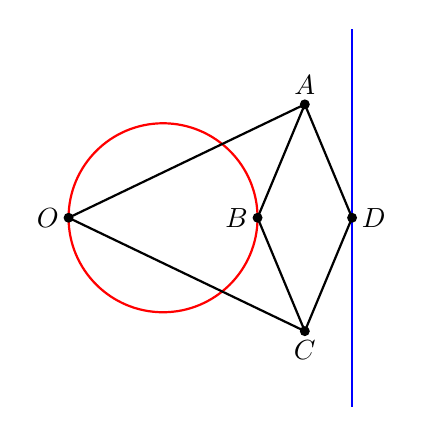
\begin{tikzpicture}[scale=1.2]

  % Circle 
  \def\r{1}
  \draw[red, thick] (0,0) circle (\r);

  % Points on/around circle
  \coordinate (O) at (-\r,0);
  \coordinate (A) at (1.5,1.2);
  \coordinate (C) at (1.5,-1.2);
  
  % Vertical line
  \coordinate (B) at (\r,0);
  \coordinate (D) at (2,0); % 2 = {2*(A.x) - (B.x)}
  \draw[blue, thick] (2,-2) -- (2,2);

  % Quadrilateral OABC
  \draw[thick] (O) -- (A) -- (B) -- (C) -- cycle;

  % Connection to D (diamond-like shape)
  \draw[thick] (A) -- (D) -- (C);

  % Mark points
  \fill (O) circle (1.5pt);
  \fill (A) circle (1.5pt);
  \fill (B) circle (1.5pt);
  \fill (C) circle (1.5pt);
  \fill (D) circle (1.5pt);

  % Labels
  \node[left] at (O) {$O$};
  \node[above] at (A) {$A$};
  \node[left] at (B) {$B$};
  \node[below] at (C) {$C$};
  \node[right] at (D) {$D$};

\end{tikzpicture}
